\documentclass[slovak,a4paper,11pt]{article}

\usepackage[utf8]{inputenc}
\usepackage{graphicx}
\usepackage{booktabs}
\usepackage{array}
\usepackage{paralist}
\usepackage{verbatim}
\usepackage{subfig}
\usepackage{amsmath}
\usepackage{index}
\usepackage{cite}
\usepackage[slovak]{babel}
\usepackage{fancyhdr}
\pagestyle{fancy}

\usepackage{sectsty}
\allsectionsfont{\sffamily\mdseries\upshape}

\usepackage[nottoc,notlof,notlot]{tocbibind}
\usepackage[titles,subfigure]{tocloft}
\renewcommand{\cftsecfont}{\rmfamily\mdseries\upshape}
\renewcommand{\cftsecpagefont}{\rmfamily\mdseries\upshape}

\title{Počítačové hry, ktoré učia programovať}
\author{Samuel Suja \\ ID: 111700 \\ Fakulta informatiky a informačných technológií STU}
%\date{}

\begin{document}
\maketitle
\tableofcontents

\begin{abstract}

Online vyučovanie sa v súčasnej situácií stalo nenahraditeľnou súčasťou študentského života. Niekedy však vedomosti zo školy nestačia na to, aby študenti vedeli všetko, čo potrebujú. V takom prípade je najlepšou možnosťou samoštúdium. Jednou z metód samoučenia je aj hranie počítačových hier. Napriek tomu že ich veľa ľudí berie ako stratu času, počítačové hry nás dokážu naučiť veci ako cudzie jazyky, logiku, históriu, a podobne. V tomto článku sa budeme venovať konkrétne takým počítačovým hrám, ktoré nás dokážu naučiť programovať, alebo nám aspoň vysvetliť základné princípy programovania. Zameriame sa na hry, ktoré sú založené na vykonávaní úloh pomocou písania alebo zoraďovania kódu, alebo ktoré obsahujú prvkypodobné samotnému programovaniu. Tými hrami budú ToonTalk, LightBot, LeekWars a CodinGame, ktoré vedia pomôcť programátorom v rôznych oblastiach ich profesie.

\end{abstract}

\section{Úvod}

Hry umožňujú hráčom zažiť, vyskúšať, alebo sa naučiť rôzne zručnosti, a zároveň sa pri tom zabávať \cite{burgos2007re}. Pomocou hier môžeme študentom ukázať nové riešenia problémov zábavným, ale zároveň efektívnym spôsobom. Pre študentov, ktorí majú problémy s pochopením niektorých tém v škole, môžu práve počítačové hry poskytnúť nový pohľad na učivo, a v niektorých prípadoch byť aj lepšou alternatívou pre vysvetlenie ťažšieho učiva \cite{seng2014computer}. Aj ak hry nie sú použité pre vzdelávanie v školskom prostredí, môžu sa k nim študenti dostať vo svojom voľnom čase a naučiť sa niečo naviac. V tomto článku sa bližšie pozreme na hry ktoré dokážu ľudí naučiť programovať, riešiť logické problémy, alebo pracovať s umelou inteligenciou; konkrétne hry ToonTalk, LightBot, LeekWars a CodinGame. Nakoniec si ukážeme, ako by sme mohli vytvoriť vlastnú hru, ktorá zlepšuje programátorské zručností hráčov.

%ToonTalk
\section{ToonTalk}
\subsection{Čo je ToonTalk?}
ToonTalk je programovací jazyk, ktorého kód môžeme vidieť v podobe interaktívneho animovaného sveta \cite{kahn1999computer}. K dispozícií máme prázdne pole a niekoľko objektov, ktoré je možné na toto pole umiestniť tak, aby sme z nich vytvorili funkčný program. Každý objekt má svoju vlastnú funkciu a zároveň dokáže komunikovať a spolupracovať s inými objektmi umiestnenými na poli. Animované nie sú len ikony týchto objektov, ale aj samotné činnosti ktoré vykonávajú a ich vzájomné vzťahy. Celý proces fungovania programu je ukázaný na obrazovke a použivateľ môže v reálnom čase sledovať ako jeho program pracuje. \\
\begin{center}
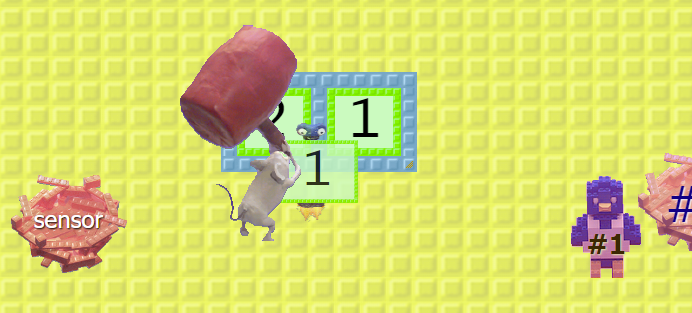
\includegraphics[scale=0.4]{toontalkmain}
\\ Obr. 1: ToonTalk v akcii: Myš zvyšuje číslo o 1
\end{center}
\subsection{Priebeh hry}
Základom ToonTalku sú samotné objekty, ktoré zastupujú príkazy a funkcie štandardných programovacích jazykov. Medzi ne patria:
\begin{itemize}
\item Čísla (ang. Numbers) - slúžia ako vstupy do aritmetických operácií
\item Škatule (ang. Boxes) - slúžia na ukladanie objektov
\item Vtáky a hniezda (ang. Birds and nests) - vedia posielať správy
\item Váhy (ang. Scales) - slúžia na porovnávanie objektov a hodnôt
\item Senzory (ang. Sensors) - rozpoznávajú kliknutia alebo stlačenia kláves
\item Funkčné vtáky (ang. Function birds) - vykonávajú funkcie so vstupnými škatuľami
\item Prehliadačové prvky (ang. Browser elements) - umožňujú prácu s obrázkami a textom z iných webových stránok
\item Roboti (ang. Robots) - vieme ich naučiť vykonávať prácu v našom programe
\end{itemize}
S týmito objektami vieme komunikovať a presúvať ich pomocou kurzoru, no máme k dispozícií dva ďalšie nástroje:
\begin{itemize}
\item Čarovná palička (ang. A Magic Wand) - dokáže skopírovať objekty
\item Vysávač Dusty (ang. Dusty the Vacuum) - slúži na odstraňovanie objektov z poľa
\end{itemize}
Cez hlavné menu ToonTalku sa dá dostať na webovú stránku, ktorá podrobne vysvetľuje ako všetky objekty fungujú, a zároveň poskytuje interaktívny návod na vyskúšanie funkčnosti všetkých objektov.
\vspace{1cm}
\begin{center}
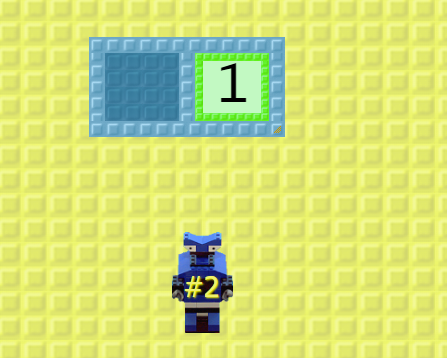
\includegraphics[scale=0.5]{toontalkrobot1}
\\ Obr. 2: Robot naprogramovaný na to, aby pripočítaval 1 k číslu v škatuli naľavo ak je v škatuli napravo číslo 1 
\\
\vspace{1cm}
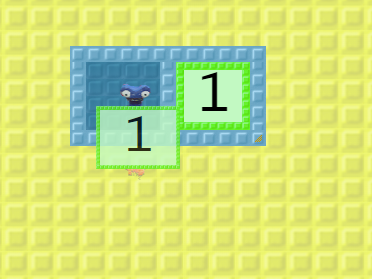
\includegraphics[scale=0.5]{toontalkrobot2}
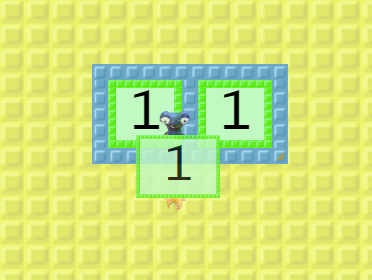
\includegraphics[scale=0.5]{toontalkrobot3}
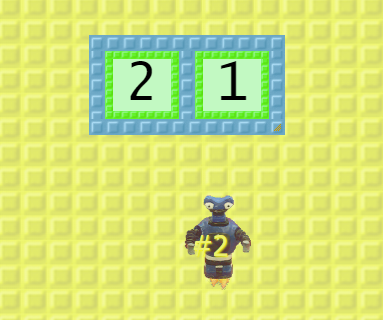
\includegraphics[scale=0.5]{toontalkrobot4}
\\ Obr. 3-5: Robot vykonáva svoju úlohu
\\
\vspace{1.5cm}
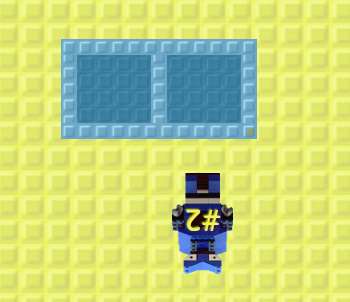
\includegraphics[scale=0.5]{toontalkrobot5}
\\ Obr. 6: V škatuli napravo nie je číslo 1, takže robot svoju prácu nevykonáva (na obrázku je preto prevrátený)
\end{center}
\subsection{Výhody a nevýhody}
Výhody:
\begin{enumerate}
\item ToonTalk umožňuje vidieť program v akcií: vidíme ako sa príkazy a funkcie vykonávajú v reálnom čase
\item Pre človeka, ktorý nikdy neprogramoval, je jednoduchšie vidieť ako jeho program funguje predtým ako to začne prepisovať do kódu
\item Objekty sa dajú rýchlo a jednoducho pridať, vymazať, alebo upraviť v pracovnom poli 
\item ToonTalk je zadarmo a dá sa spustiť cez skoro každý webový prehliadač bez potreby sťahovania
\item Správne urobený program môže slúžiť aj na naučenie iných vecí ako programovania
\end{enumerate}
Nevýhody:
\begin{enumerate}
\item Správne naprogramovať robotov je zložitejšie ako sa na prvý pohľad zdá. Pre ľudí, ktorí majú s programovaním skúsenosti, to môže byť zbytočne zdĺhavé
\item Zložitejšie programy je ťažké naprogramovať tak, aby všetko fungovalo bezchybne
\item Pri veľkom počte objektov je ťažké sa na poli zorientovať.
\item Poslednú aktualizáciu dostal ToonTalk na konci roku 2016, takže bugy, ktoré sa dodnes nachádzajú v aplikácií, nebudú už pravdepodobne nikdy odstránené
\end{enumerate}
\subsection{Zhodnotenie}

%LightBot
\section{LightBot}
\subsection{Čo je LightBot?}
LightBot nie je hra, ktorá dokáže hráčom priamo vysvetliť princípy programovania. Jadro tejto hry spočíva v skladaní príkazov do algoritmov s cieľom dostať sa do ďalšej úrovne \cite{combefis2016learning}. V hre ovláda hráč robota, ktorý sa vie pohybovať po políčkach a vykonávať rôzne úlohy. Aby hráč postúpil do ďalšej úrovne, musí pomôcť robotovi zapáliť svetlá na všetkých políčkach zafarbených modrou farbou. Toto hráč docieli poskladaním postupnosti príkazov do procedúry main, ktoré má robot vykonať aby úspešne dokončil úroveň. \\
\begin{center}
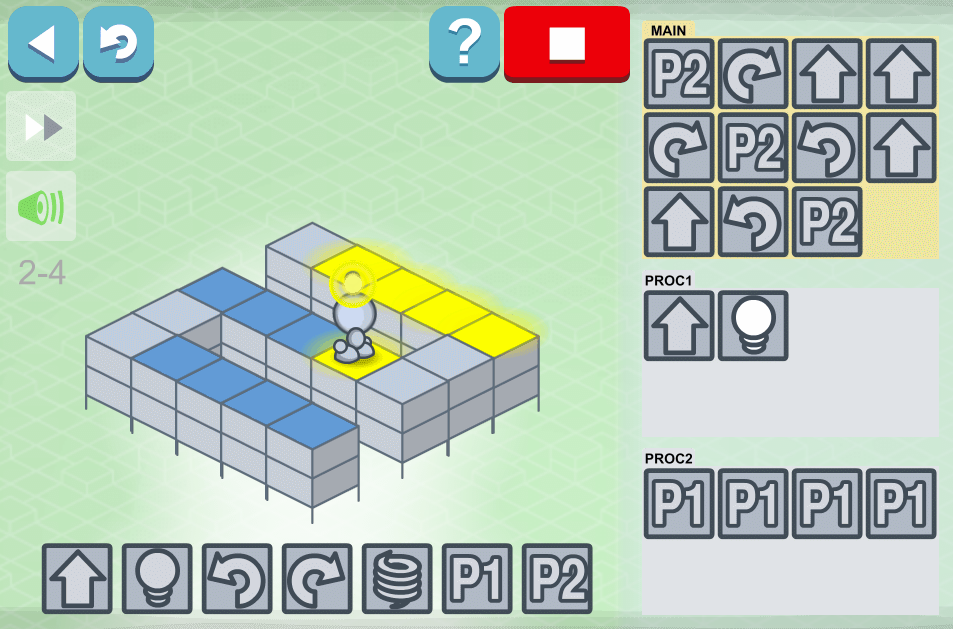
\includegraphics[scale=0.3]{lightbotmain}
\\ Obr. 7: Úspešné riešenie úrovne 2-4
\end{center}
\subsection{Priebeh hry}
Cieľom hráča je zapáliť všetky svetlá (políčka zafarbené modrou farbou) na hracom poli. Na pravej strane obrazovky sa nachádza procedúra main: po stlačení tlačidla na spustenie robota vykoná LightBot príkazy zadané v tejto funkcií. Main má však limit 12 príkazov, čo núti hráča v niektorých úrovniach nájsť to najefektívnejšie riešenie. V neskorších úrovniach pribudnú ďalšie procedúry, ktoré majú limit len 8 príkazov, ale môžeme ich vykonať cez procedúru main. To nám umožňuje vykonať niekoľkonásobne viac príkazov, ale zároveň robí riešenie úrovne zložitejším. \\
Na dolnej strane obrazovky sa nachádzaju samotné príkazy, ktoré môže robot vykonať. Medzi ne patrí:
\begin{itemize}
\item Pohyb dopredu
\item Zapálenie alebo zhasnutie svetla na políčku
\item Otočenie doľava
\item Otočenie doprava
\item Skok - špeciálny pohyb dopredu, ktorým sa dá pohybovať medzi políčkami rôznych výšok
\item Procedúra - vykoná všetky príkazy vo vybranej procedúre
\end{itemize}
\subsection{Výhody a nevýhody}
Výhody:
\begin{enumerate}
\item LightBot môže hrať aj človek, ktorý nikdy neprogramoval
\item Návod je stručný a ľahko pochopiteľný
\item Hru môžu hrať aj ľudia, ktorí nechcú byť programátormi
\item LightBot zlepšuje schopnosť riešiť problémy a logické myslenie
\item Neskoršie úrovne sú výzvou aj pre skúsených programátorov
\end{enumerate}
Nevýhody:
\begin{enumerate}
\item Hráči sa neučia programovať, len zlepšujú zručnosti užitočné pri programovaní
\item Hra má len limitovaný počet úrovní
\item Aj keď sa dá LightBot hrať zadarmo, plná verzia so všetkými úrovňami je platená
\item Hráč nemá veľa možností rozvíjať kreativitu, keďže neskoršie úrovne majú väčšinou len jedno správne riešenie
\end{enumerate}
\subsection{Zhodnotenie}

%LeekWars
\section{LeekWars}
\subsection{Čo je LeekWars?}
LeekWars je online hra pre viac hráčov, v ktorej hráč bojuje so svojim pórom (ang. leek) proti pórom ostatných hráčov \cite{combefis2016learning}. Hráč si môže pre svoj pór kupovať rôzne zbrane a čipy, ktoré mu pridávajú nové schopnosti a poskytujú nové možnosti boja, alebo mu zlepšovať jeho štatistiky (napr. rýchlosť, životy, sila). Bojovaním získava pór body skúsenosti, pomocou ktorých sa mu zvyšuje úroveň a stáva sa silnejším. Hlavným problémom je však to, že ani jeden z hráčov nemá kontrolu nad svojim pórom. Tomu môže dávať príkazy len kód, ktorý každý hráč svojmu póru napíše pred tým, ako ho pošle do boja. \\
\begin{center}
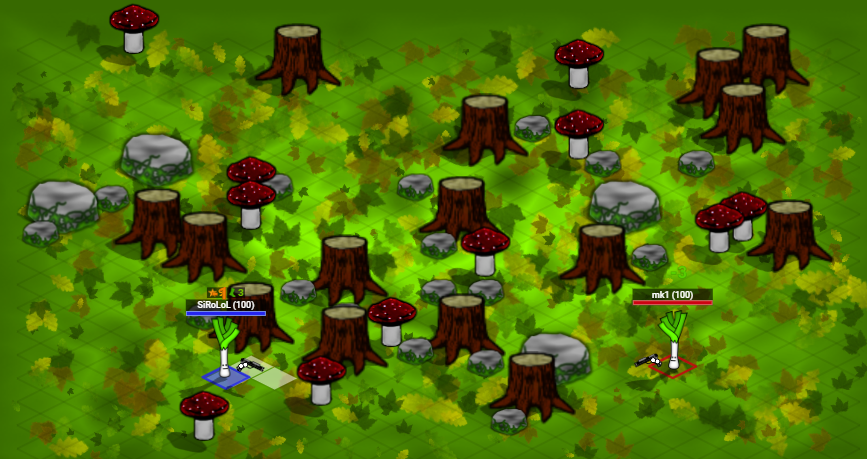
\includegraphics[scale=0.4]{leekwarsmain}
\\ Obr. 8: Pór hráča (vľavo) bojuje proti póru iného hráča (vpravo)
\end{center}
\subsection{Priebeh hry}
Hráč si najprv vytvorí svoj pór, ktorý začína na prvej úrovni. Ku svojmu póru dostane základný kód (Obr. 9), ktorý môže už od začiatku upraviť v editore kódu (Obr. 10). Kód je písaný v jazyku JavaScript, pričom sú k nemu pridané nové funkcie z LeekWars potrebné na interakciu s herným prostredím (napr. useWeapon, moveToward).
\begin{center}
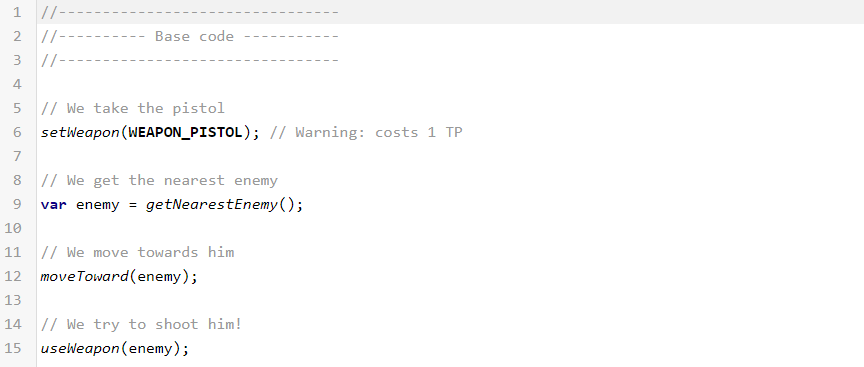
\includegraphics[scale=0.4]{leekwarscode1}
\\ Obr. 9: Základný kód, ktorý hráč dostane na prvej úrovni
\end{center}
\begin{center}
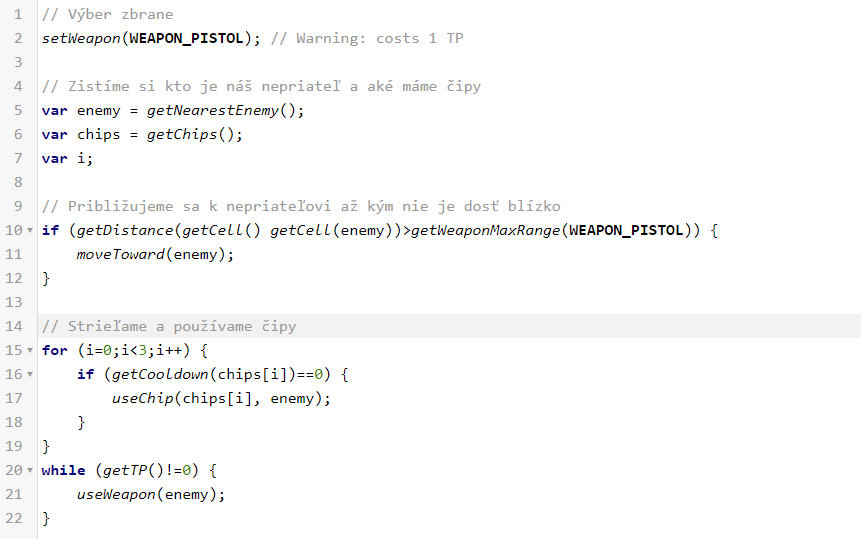
\includegraphics[scale=0.4]{leekwarscode2}
\\ Obr. 10: Jednoduchý kód pre pór s 3 čipmi a pištoľou
\end{center}
Ďalej má hráč sprístupnený trh (ang. Market), kde si môže nakúpiť nové zbrane a čipy za hernú menu zvanú Habs. Každá vec na trhu sa však dá kúpiť až po dosianutí určitej úrovne. Herné peniaze aj body skúsenosti potrebné na nákup nových zbraní môže hráč získať v záhrade (ang. Garden), kde môže bojovať proti iným hráčom. Ďalej môže hráč získať rôzne trofeje, pozrieť sa na rebríček najlepších hráčov, alebo si pozrieť návod na LeekWars kódovanie.\\
Samotný boj s hráčmi prebieha tak, že póry hráčov sa po kolách striedajú
\subsection{Výhody a nevýhody}
Výhody:
\begin{enumerate}
\item LeekWars môže byť zábava aj pre neprogramátorov, stačí používať základný kód a upravovať len svoje zbrane, čipy a schopnosti
\item Hra je skvelá na trénovanie programovania umelej inteligencie
\item Keďže základom programovania pórov je JavaScript, môžu sa hráči pomocou LeekWars naučiť v tomto jazyku pracovať 
\item LeekWars je zadarmo a dá sa jednoducho spustiť z webového prehliadača
\item Pri hre môže hráč stráviť veľa času, nakoľko môže zvyšovať úroveň pórov až do úrovne 301 a môže postupne vytvoriť až 4 póry
\end{enumerate}
Nevýhody:
\begin{enumerate}
\item Ak sa hráč nesnaží neustále vylepšovať kód svojho póru, hra sa stáva repetitívnou
\item Bojové mapy sa niekedy môžu zle vygenerovať, čo znamená, že sa hráči k sebe nemôžu dostať a bojovať
\item Niektoré časti hry (hlavne errory) nie sú preložené do angličtiny, a ak hráč nevie po francúzsky, je opravovanie chýb v kóde dosť náročné
\item Väčšina hráčov LeekWars už aktívne nehrá, takže je problém nájsť spoluhráčov do tímových bitiek
\end{enumerate}
\subsection{Zhodnotenie}

%CodinGame
\section{CodinGame}
\subsection{Čo je CodinGame?}
CodinGame je online hra, v ktorej je hráčovým cieľom naprogramovať svojho agenta tak, aby splnil požiadavky na prejdenie úrovňou \cite{combefis2016learning}. Hráč si môže vybrať jeden z dostupných jazykov, v ktorom bude programovať, a napíše svoj kód tak, aby jeho agent úspešne prešiel cez všetky testovacie situácie. Každá testovacia situácia vloží agenta do iných podmienok, ale hráč musí pre všetky testovacie situácie použiť ten istý kód. Podmienky niektorých z týchto testov sú hráčovi predom známe, no niektoré sú skryté, aby hráč dospel k všeobecnému riešeniu.\\
\begin{center}
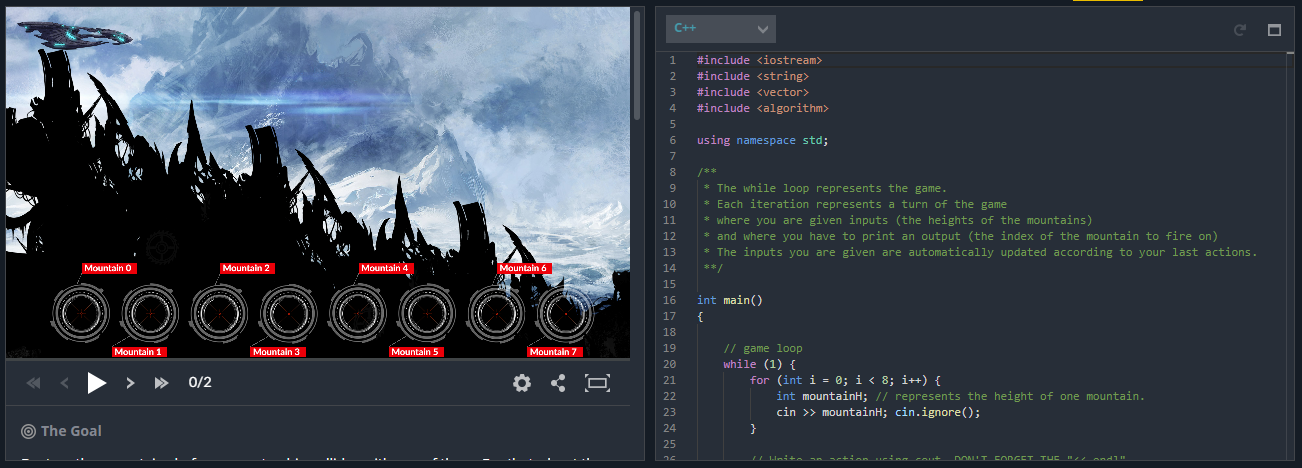
\includegraphics[scale=0.28]{codingamemain}
\\ Obr. 11: Začiatočnícka úroveň "The Descent". Na ľavej strane sa nachádza úroveň, ktorej cieľom je zničiť s loďou všetky hory bez toho, aby do nich loď narazila
\end{center}
\subsection{Priebeh hry}
Na začiatku si hráč vyberie jednu z dostupných úrovní. Tieto úrovne sú rozdelené do štyroch kategórií podľa ich náročnosti: ľahké, stredné, ťažké a veľmi ťažké. Po spustení sa na obrazovke objaví okno s kódom, okno pre výber jednej z testovacích situácii, a okno so samotnou úrovňou. Hráčovi je v kóde pomocou komentárov vysvetlené, čo kód robí, a hráč môže ďalej k riešeniu pristupovať akýmkoľvek spôsobom. Na obrazovke vidí hráč svojho agenta a prostredie, v ktorom sa nachádza. Pod obrazovkou sa nachádzajú podmienky prehry a podmienky úspešného dokončenia úrovne. Hráč si ďalej môže svoj kód spustiť len v jednej z testovacích situácií, alebo ho môže naraz spustiť vo všetkých. Ak hráč úspešne splní podmienky dokončenia v každej testovacej situácií, úroveň je úspešne dokončená a hráč je odmenený bodmi skúseností.\\
\begin{center}
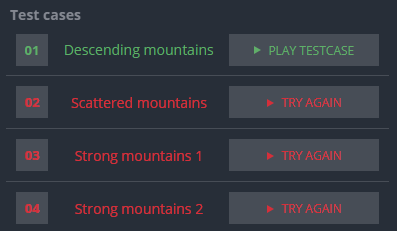
\includegraphics[scale=0.6]{codingametest}
\\ Obr. 12: Testovacie situácie úrovne "The Descent". Hráč splnil podmienky len v jednej z nich, takže úroveň zatiaľ úspešne nedokončil
\end{center}
\subsection{Výhody a nevýhody}
Výhody:
\begin{enumerate}
\item CodinGame je zadarmo a dá sa hrať priamo na webovej stránke
\item Pre skúsených programátorov je hra skvelá na trénovanie riešenia problémov
\item Hra často organizuje rôzne súťaže pre developerov a pridáva nové úrovne
\item Hráč má na výber z veľkého množstva jazykov
\item Hráči si môžu vyskúšať aj rôzne úrovne vytvorené inými ľuďmi, alebo vytvoriť svoje vlastné
\item CodinGame oznamuje všetkým hráčom, ktorí ho majú momentálne spustený, ak práve niekto túto hru streamuje
\item Okrem samotnej hry poskytuje CodinGame aj možnosť nájsť si prácu v IT spoločnosti ako Google, Facebook alebo Dropbox
\end{enumerate}
Nevýhody:
\begin{enumerate}
\item Ak hráč neovláda základy nejakého programovacieho jazyku, v CodinGame sa ich nenaučí
\item Zo začiatku je trochu ťažké sa zorientovať v použivateľskom rozhraní stránky
\item Hráč sa musí najprv zaregistrovať, čo mu môže prekážať ak chce CodinGame len vyskúšať pred tým, ako sa naozaj zaregistruje
\end{enumerate}
\subsection{Zhodnotenie}

\section{Záver}

\bibliography{referencie}
\bibliographystyle{plain}

\end{document}
